\chapter{Programmbeschreibung}\label{ch:programmbeschreibung}

\section{Programmablaufplan}\label{sec:pap}
Die folgenden Abbildungen beschreiben Teile des Programms.

Abbildung~\ref{fig:diagramm1} und ~\ref{fig:diagramm2} zeigen den Ablauf des Gruppenwechsels.

In Abbildung~\ref{fig:diagramm3} wird die Ermittelung der Leistungsbezeichnungen visualisiert.


\begin{figure}[!h]
    \centering
    \includegraphics[scale=0.9,width=\textwidth,height=\textheight,keepaspectratio]{images/Gruppenwechsel-PAP.pdf}
    \caption{
        Veranschaulichung des Gruppenwechsels
    }
    \label{fig:diagramm1}
\end{figure}

\begin{figure}[!h]
    \centering
    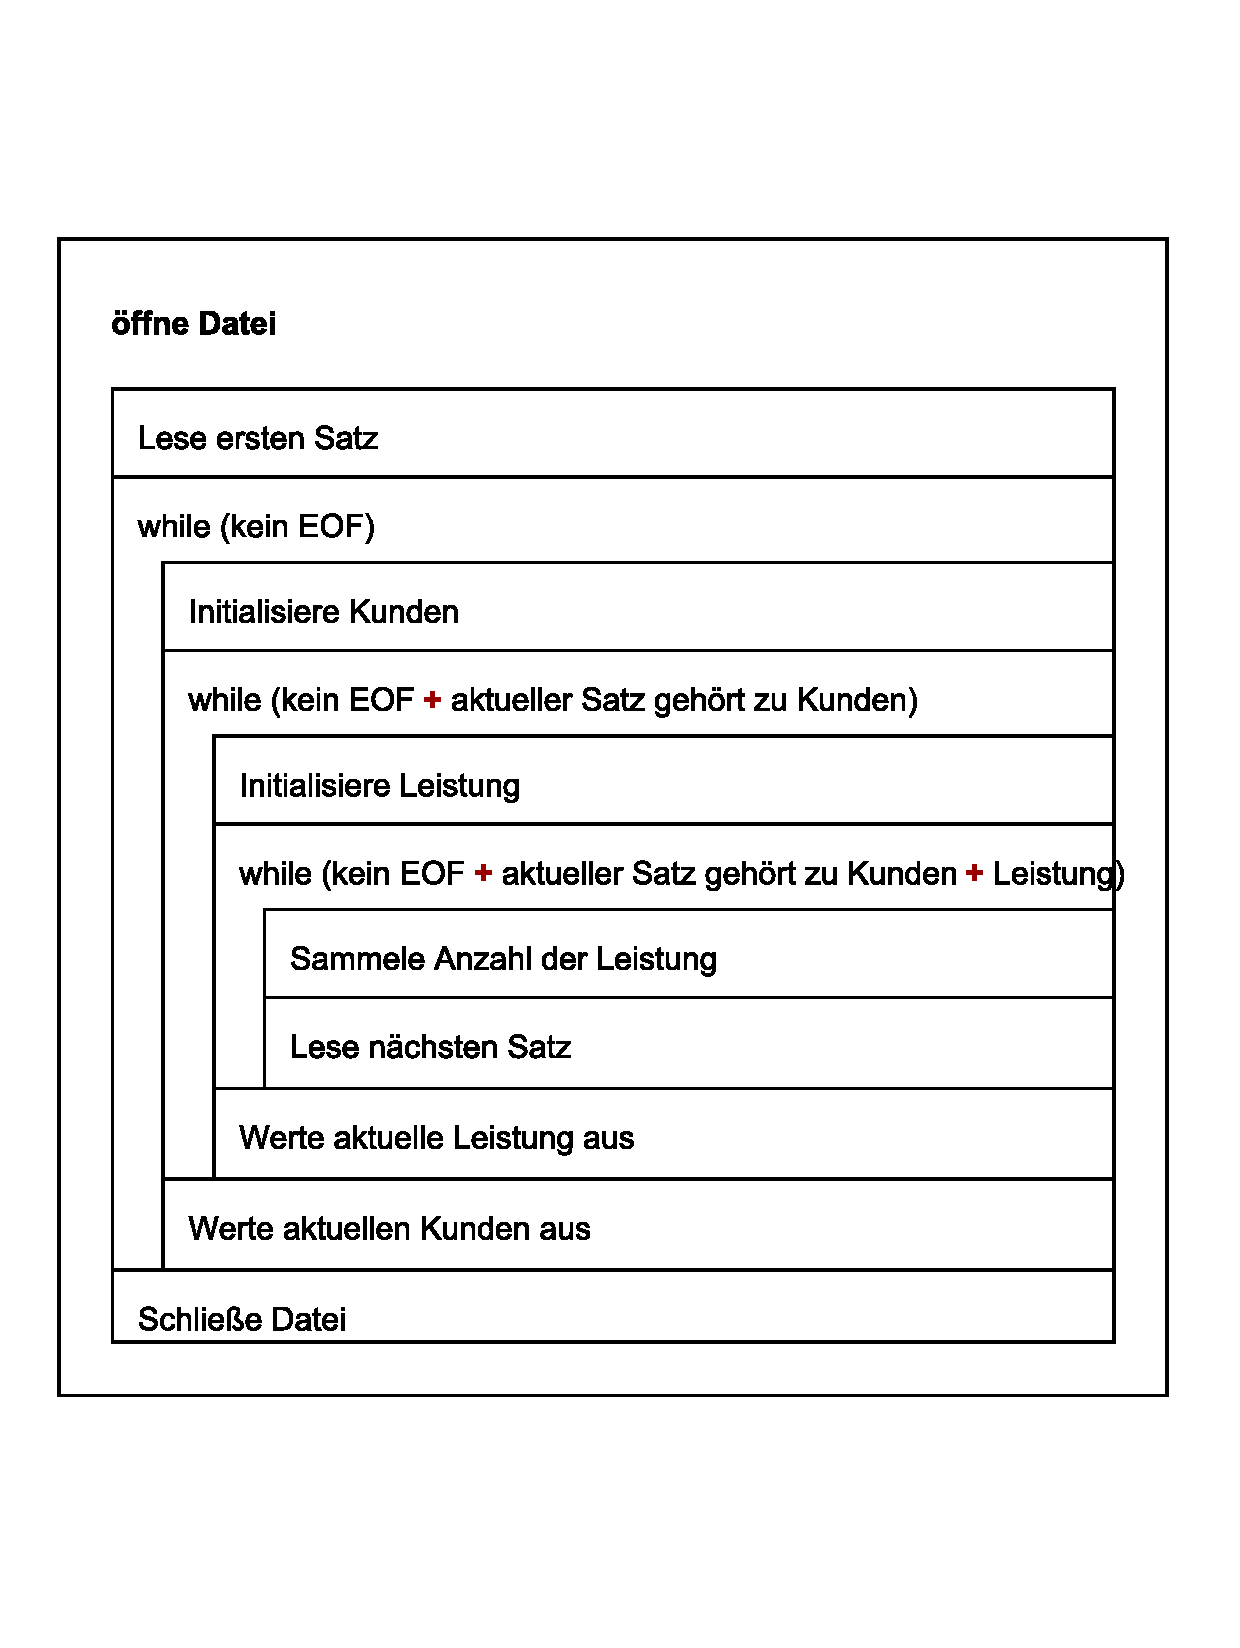
\includegraphics[width=\textwidth,height=\textheight,keepaspectratio]{images/Gruppenwechsel-NSD.pdf}
    \caption{
        Veranschaulichung des Gruppenwechsels II
    }
    \label{fig:diagramm2}
\end{figure}

\begin{figure}[!h]
    \centering
    \includegraphics[width=\textwidth,height=\textheight,keepaspectratio]{images/Erhalte_Leistungsbezeichnung-PAP.pdf}
    \caption{
        Ablauf der Ermittlung der Leistungsbezeichnugnen
    }
    \label{fig:diagramm3}
\end{figure}



\section{Entwicklungsdokumentation}\label{sec:entwicklerdokumentation}
Es wurden grundsätzlich sprechende Namen für Variablen, Abschnitte und Paragrafen gewählt. Außerdem sind \texttt{DISPLAY} Statements welche zum Debuggen genutz wurden erhalten geblieben. Mit diesen ist der Programmablauf leichter nachzuvollziehen.

Daher bedarf es nur geringer Dokumentation.
Die Funktionen der einzelnen Paragrafen sind in Tabelle~\ref{tab:prog-strukt} beschrieben.


\definecolor{fhfarbe}{HTML}{51B2AC}
\definecolor{fhfarbe2}{HTML}{4FAEAB}
\begin{table}[!htb]
    \centering
    \rowcolors{2}{black!5}{white}
    \begin{tabularx}{\textwidth}{X | X }
       \rowcolor{fhfarbe!25}
       Bezeichnung                             & Beschreibung             \\
%       \hline
       \rowcolor{fhfarbe!10}
       MAIN-PROCEDURE & Hauptablauf welcher den Gruppenwechsel delegiert \\
       PREPERATION & Spiegelt den Vorlauf zum einlesen einer Datei wieder und öffnet die Einlsese- (JOURNAL.txt) und Auslesedatei (INVOICE.txt) \\
       CUSTOMER-PREPERATION & Wertet den akutellen Einlesesatz aus und initialisiert daraus einen Kunden \\
       SERVICE-PREPERATION & Wertet den aktuellen Einlesesatz weiter aus und initialisiert daraus eine Leistung \\
       INDIVIDUAL-PROCESSING & Wertet den aktuellen Einlesesatz aus und zählt die Vorkommensanzahl einer Leistung hoch \\
       READ-NEXT-LINE & Liest, wenn möglich, die nächste Zeile des Jounrals ein \\
       SERVICE-COMPLETION & Wertet die aktuelle Leistung aus indem der Gesamtbetrag der Leistung berechnet und mit allen relevanten Leistungsdaten in die Rechnung geschrieben wird \\
       CUSTOMER-COMPLETION & Wertet den aktuellen Kunden aus indem der Gesamtbetrag des Kunden in die Rechnung geschrieben und ein Ende gekennzeichnet wird \\
       COMPLETION & schließt Einlese- und Auslesedatei \\
       
       \rowcolor{fhfarbe!10}
       GET-SERVICE-TERM & Ermittelt anhand der Leistungs-ID durch einlesen des Leistungsglossar die Leistungsbeschreibung \\
       CHECK-LINE & Überprüft, ob die aktuell aus dem Glossar eingelesene Leistungs-ID mit der zu überprüfenden Leistungs-ID übereinstimmt \\
       NEXT-LINE & Liest, wenn möglich die nächste Zeile des Glossars ein\\
       DISPLAY-JOURNAL & Debugeinheit zum ausgeben der aktuell eingelesenen Daten \\
    \end{tabularx}
    \caption{Aufgaben der einzelnen logischen Einheiten.}\label{tab:prog-strukt}
\end{table}
